\documentclass{apuntes}

\title{MNEDO}
\author{Pedro Valero \& Jorge Martín}
\date{15/15 C1}
% Paquetes adicionales
\usepackage{tikztools}
\usepackage{fastbuild}
\usepackage{tikz-3dplot}
\usepackage{fancysprefs}

\bibliographystyle{plainnat}

\usetikzlibrary{arrows}
% --------------------

\precompileTikz

\begin{document}
\pagestyle{plain}
\maketitle

\tableofcontents


\chapter{Preliminares}

\section{Problemas de valor inicial. (PVI)}

A lo largo de este curso estudiaremos problemas de valor inicial, que no son más que ecuaciones diferenciales ordinarias (EDOs) junto con un dato inicial, necesario para resolver adecuadamente la ecuación. Se trata de sistemas de la forma:
\[\begin{cases}
		y'(x)=f(x,y(x)) & x∈[a,b]\\
		y(a)=y_a
\end{cases}\]
done $y(x)$ es una función del tipo
\[\appl{y}{ℝ}{ℝ^d}\]
\[y(x)=(y_1(x), …, y_d(x))\]

Por tanto $f$ quedará definida como:
\[\appl{f}{ℝ×ℝ}{ℝ^d} \]
\[f(x,y) = (x,y(x))\]

Como notación muchas veces consideraremos $y(x)=y$, del mismo modo que $y(a)=y_a$ con $a$ un valor dado.

\begin{remark}
	En el curso trabajaremos con funciones $f∈C\left( [a,b] × ℝ^d \right)$
\end{remark}


\begin{defn}[Función Lipschitz]
	Una función $f$ será Lipschitz en la segunda variable existe una constante $L$ tal que:
	\[∀x ∈ [a,b], ∀y_1,y_2 ∈ℝ^d \ \md{f(x,y_1) - f(x,y_2)} ≤ L\md{y_1-y_2}\]
\end{defn}

Vamos a ver en qué situaciones este tipo de problemas tienen solución única:

\begin{theorem}[Teorema de Picard]
	\label{TeoremaPicard}
	Sea $Ω=[a,b]×ℝ^d$, si $f$ es continua en $Ω$ y Lipschitz en la segunda variable; entonces \textbf{el PVI tiene una única solución} $y∈C'\big([a,b] × ℝ^d\big)$
\end{theorem}

\begin{proof}
	\textbf{Vamos a demostrar primero la existencia de la solución}:
	Para ello haremos uso de las iteradas de Picard, definidas mediante:

	\[y(x)=y_a+\int_a^x f(s,y(s))ds\]

	Si definimos la aplicación $T_y = y_a + \int_a^x f(s,y(s))ds$, encontrar la solución $y$ es qeuivalente a encontrar un punto fijo de dicha aplicación. Vamos a ello.

	\begin{enumerate}
		\item \textbf{Construimos la secuencia de funciones $\{ y_n(x) \}_{n=0}^∞$}:
		\[y_{n+1}(x) = y_a + \int_a^x f(s,y_n(s)) ds\]
		\[n=0,1,… \text{\ y \ } y_0(x)=y_a\]
		Cada función $y_n$ es continua (es una constante más una función continua).

		\item \textbf{Debemos probar que $∃y ∈ C([a,b])$ tal que}:
		\[y_n \longrightarrow y \text{\ uniformemente}\]
		Que es equivalente a decir que $\lim_{n \to ∞} \md{y_n - y}_{L^∞[a,b]} = 0$. Donde $\md{f}_{L^∞[a,b]} = \max_{x ∈ [a,b]}\md{f(x)}$, denota la norma infinito de $f$.
	\end{enumerate}

	Antes de continuar vamos a recordar el Test M de Weierstrass:

	\begin{theorem}[Test M de Weierstrass]
		\label{TestMWeierstrass}
		Sea $\{f_n\}_{n=0}^∞$ una sucesión de funciones definidas en un dominio $Ω$ con valores en $ℝ$, si existe una sucesión de números $M_n$ tal que:
		\begin{enumerate}
			\item $\abs{f_n} < M_n \text{,\ } ∀x∈Ω$
			\item $\sum_{n=0}^∞ M_n < ∞$
		\end{enumerate}

		Entonces existe una función $g$ tal que:
		\[g_n(x) = \sum_{n=1}^N f_n\]
		\[g_n \xrightarrow[n \rightarrow ∞]{} g \text{,\ uniformemente en\ } x\]
	\end{theorem}

	¿Cómo vamos a usar esto para conseguir ver que $y_n \rightarrow y$?.\\
	Primero vamos a reescribir $y_n$ como (sabiendo que tomamos $y_a=y_0$) una suma telescópica:

	\[y_{n+1} = y_a + \sum_{k=0}^n y_{k+1} - y_k\]
	Para el caso $n=1$: $y_2 = y_a + (y_1 - y_0) + (y_2 - y_1) = y_2$.

	Ahora vamos a aplicar el test M de Weierstrass:

	Las $f_k$ que aparecen en el enunciado de \ref{TestMWeierstrass} serán $(y_{k+1} - y_k)$, si demuestro que $∃{M_k}$ tales que:

	\[\abs{y_{k+1}-y_k} < M_k \text{,\ } ∀x∈[a,b]\]
	\[\text{y que\ } \sum_k M_k < ∞ \text{, entonces } ∃y \text{ tal que:}\]
	\[y_n \rightarrow y \text{ uniformemente}\]

	Vamos a encontrar dichos $M_k$:

	\begin{lemma}
		\[\abs{y_{k+1} - y_k} ≤ \frac{C(y_a)}{L}\frac{(L(x-a))^{k+1}}{(k+1)!}\]
	\end{lemma}
	\begin{proof}
		Vamos a proceder a demostrar el lema usando inducción, así que vamos a ver que es cierto para $k=0$:

		\[\abs{y_1-y_0}=\abs{\int_a^x f(s,y_a) ds} ≤ \int_a^x \abs{f(s,y_a)} ds ≤\]
		\[≤ \md{f(x,y_n)}_{L^∞[a,b]} (x-a) = C(y_n) (x-a)\]

		Ahora supondremos que el lema es cierto para $k-1$ para poder demostrarlo para $k$:

		\[\abs{y_{k+1}-y_k} = \abs{\int_a^x f(s,y_k(s)) - \int_a^x f(s,y_{k-1}(s))} ds ≤\]
		\[≤ \int_a^x \abs{f(s,y_k(s)) - f(s,y_{k-1}(s))} ds \underbrace{≤}_{\mathclap{f \text{ Lipschitz en 2ª variable}}} L \int_a^x \abs{y_k(s) - y_{k-1}(s)} ds ≤\]
		\[\underbrace{≤}_{\text{hip. inducción}} L \int_a^x \frac{C(y_a)}{L} \frac{(L(s-a))^k}{k!} ds ≤ C(y_a)\frac{L^k}{k!}\int_a^x (s-a)^k ds ≤\]
		\[≤ C(y_a) \frac{L^k}{(k+1) k!}(x-a)^{k+1}\]
	\end{proof}

	Volviendo a la demostración de \ref{TeoremaPicard} recordemos que queríamos encontrar los $M_k$ necesarios para ver la convergencia de nuestras $y_k$. Gracias al lema que acabamos de demostrar y al test M de Weierstrass \ref{TestMWeierstrass} podemos afirmar:

	\[\abs{y_{k+1}-y_k} ≤ \frac{C(y_a)}{L} ≤ \frac{C(y_a)}{L}\frac{(L(x-a))^{k+1}}{(k+1)!} = M_k\]

	Los siguiente es verificar la segunda hipótesis de \ref{TestMWeierstrass}:

	\[M_k = \frac{C(y_a)}{L}\frac{[L(x-a)]^{k+1}}{(k+1)!} \underbrace{=}_{s=L(x-a)} \frac{C(y_a)}{L}\frac{s^{k+1}}{(k+1)!}\]

	Sabiendo que $e^x = \sum_{k=0}^∞ \frac{x^k}{k!}$:

	\[\sum_{k=0}^∞ M_k = \frac{-C(y_a)}{L} (1 - \frac{C(y_a)}{L} \sum_{k=0}^∞ \frac{s^k}{k!}) = \frac{C(y_a)}{L} (e^s - 1) < ∞\]

	Luego aplicando el test M de Weierstrass \ref{TestMWeierstrass}:
	\[∃y \text{ tal que: } y_n\rightarrow y \text{ uniformemente en} [a,b]\]

	\begin{enumerate}
		\setcounter{enumi}{3}
		\item Por tanto hemos probado que $∃y$ tal que $y_n \rightarrow y$ uniformemente, y por lo tanto $y∈C([a,c])$ (sabemos que la convergencia uniforme de una sucesión de funciones continuas hace que la función a la que se converge sea continua).

		\item
			\[y_{n+1} = y_a + \int_a^x f(s,y_n(s))ds \underbrace{\longrightarrow}_{n \rightarrow ∞} y = y_a + \int_a^x f(s,y(s))ds\]
			Como $f∈C([a,b])$ y $y_n$ son continuas, está claro que $y$ es continua. De modo que \textbf{\underline{hemos demostrado que existe solución}} $y∈C([a,b])$.
	\end{enumerate}

	Lo que \underline{nos queda es demostrar la unicidad} de la solución:

	Supongamos que existen dos soluciones distintas $y,\tilde{y} ∈ C([a,b])$:
	\[y(x) = y_a + \int_a^x f(s,y(s))ds\]
	\[\tilde{y}(x) = y_a + \int_a^x f(s,\tilde{y}(s))ds\]
	\[\abs{y(x) - \tilde{y}(x)} = \int_a^x \abs{f(s,y(s)) - f(s,\tilde{y}(s))} ds ≤\]
	\[≤ L \int_a^x \abs{y(s) - \tilde{y}(s)} ds \]

	Definimos $g(x)=\int_a^x \abs{y(s) - \tilde{y}(s)} ds$:

	\begin{equation}
		\label{eqDemPicard}
		g'(x) = |y(x) - \tilde{y}(x)| \leq Lg(x); \ g'(x)e^{-L(x-a)} \leq Lg(x)e^{-L(x-a)}
	\end{equation}

	Seguimos:
	\[\left( g(x)e^{-L(x-a)} \right)^{'} = g'(x) e^{-L(x-a)} - Lg(x) e^{-L(x-a)}\]
	\[g'(x) e^{-L(x-a)} = \left( g(x)e^{-L(x-a)} \right)^{'} + Lg(x) e^{-L(x-a)}\]

	Usando \ref{eqDemPicard}:
	\[\left( g(x)e^{-L(x-a)} \right)^{'} + Lg(x) e^{-L(x-a)} ≤ Lg(x) e^{-L(x-a)}\]
	\[\left( g(x)e^{-L(x-a)} \right)^{'} ≤ 0\]

	Si integramos a ambos lados entre $a$ y $X$:
	\[g(X) e^{-L(x-a)} ≤ g(a) = 0 \text{ por como hemos definido } g\]

	Por tanto:
	\[g(X) = \int_a^X \abs{\tilde{y}(x) - y(x)} dx = 0 \implies \tilde{y}=y\]

	Y hemos demostrado la unicidad de la solución.
\end{proof}

Lo siguiente que cabe preguntarse es cómo varía la solución de un problema de valor inicial (PVI) cuando variamos el dato inicial. Y la respuesta es que al variarlo muy poco, la solución también se altera muy poco.

\begin{theorem}[Continuidad con respecto al dato inicial]
	Sea $y' = f(x,y(x))$ un problema de valor inicial (PVI) con dos datos iniciales distintos $y_a, \tilde{y}_a$, con $f$ Lipschitz en la segunda variable y continua en $Ω=[a,b]×ℝ^d$:
	\[\md{y(x)-\tilde{y}(x)}_{L^∞[a,b]} ≤ \abs{y_a - \tilde{y}_a} e^{L(b-a)}\]
\end{theorem}
\begin{proof}
	Tomando como soluciones las que se sacan con la iterada de Picard:

	\[y(x)-\tilde{y}(x)=y_a-\tilde{y}_a + \int_a^x (f(s,y(s)) - f(s,\tilde{y}(s)))ds\]
	\[\abs{y - \tilde{y}} ≤ \abs{y_a - \tilde{y}_a} + \int_a^x \abs{f(s,y(s)) - f(s,\tilde{y}(s))} ds ≤\]
	\[≤ \underbrace{ \abs{y_a - \tilde{y}_a} + L\int_a^b \abs{y(s)-\tilde{y}(s)} ds}_{g(x)} \]

	Por tanto $g'(x) = L\abs{y(x) - \tilde{y}(x)}$. Si sobre esta última igualdad realizamos el procedimiento del factor integrante que hemos llevado a cabo al demostrar la unicidad en el teorema de Picard \ref{TeoremaPicard} llegamos a:

	\[g(x)e^{-L(x-a)} ≤ \abs{\tilde{y}_a - y_a} \implies g(x) ≤ \abs{\tilde{y}_a - y_a}e^{L(x-a)}\]

	Por último:
	\[\abs{y_(x) - \tilde{y}(x)} ≤ g(x)\]
	\[y(x) - \tilde{y}(x) ≤ \abs{\tilde{y}_a - y_a}e^{L(x-a)}\]
	\[\md{y - \tilde{y}}_{L^∞[a,b]} ≤ \abs{y_a - \tilde{y}_a} e^{L(b-a)}\]
\end{proof}

Vamos ahora a ver ejemplos donde aplicar el teorema de Picard \ref{TeoremaPicard}:

\begin{example}
	Para el problema de valor inicial (PVI) $y'(x)=\sqrt{x}$, $y(0)=0$; tenemos $f(x,y(x))=\sqrt(y)$. Esta $f$ no es Lipschitz y por tanto no cumple las hipótesis del teorema de Picard \ref{TeoremaPicard}, de hecho existen dos soluciones distintas:
	\[y_1(x) = 0\]
	\[y_2(x) = x^2\]
\end{example}


\section{Algunos ejemplos de métodos numéricos para PVI.}
Recordemos que el objetivo de este curso es encontrar soluciones a problemas de valor inicial (PVI) del tipo:

\[y'(x) = f(x,y(x)) \text{, } x∈[a,b]\]
\[y(a)=y_a\]

Lo que queremos conocer es cómo se comporta y(x) sin saber encontrar su solución. Para ello, como ya hemos visto, podemos usar las iteradas de Picard:

\[y_{n-1}(x) = y_a + \int_a^x f(s,y_n(s)) ds\]
\[y_0(x) = y_a\]

\begin{remark}
Durante este curso, al emplear los diferentes métodos numéricos usaremos versiones discretizadas de las funciones, es decir, el conjunto de valores que tomará una función $y(x)$ será sobre una serie de valores ${x_n}_{n=0}^N$ dentro del intervalo $[a,b]$, donde $x_0=a$ y $x_N=b$.
\end{remark}
En este curso la distancia entre cada muestra será igual $x_{n+1}-x_n=h=\frac{b-a}{N}$.

A continuación mencionaremos algunos métodos numéricos que estudiaremos más adelante:
\begin{itemize}
	\item \textbf{Método de Euler}
	\[y'(x) = f(x,y(x))\]
	\[y'(x_n) = f(x_n,y(x_n))\]
	Pero dado que $x$ toma valores discretos:
	\[\frac{y(x_{n+1}) - y(x_n)}{h} \implies \frac{y_{n+1} - y_n}{h} = y'(x_n) = f(x_n,y(x))\]
	Así la fórmula de recurrencia del método de Euler queda como:
	\[y_{n+1} = y_n + h·f(x,y_n)\]
	\[y_0=y_a\]

	\item \textbf{Desarrollo en serie de Taylor}
	\[y(x_{n+1}) = y(x_n+h) = y(x_n) + h·y'(x_n) + R_n =\]
	\[= y(x_n) + h·f(x_n,y(x_n)) + R_n\]

	\item \textbf{Método leap-frog}
	\[y(x_{n+2}) - y(x_n) = \int_{x_n}^{x_{n+2}} y'(x) = \int_{x_n}^{x_{n+2}} f(x,y(x))\dif x \approx (x_{n+2}-x_n)f(x_{n+1},y(x_{n+1}))\]
	donde la aproximación se ha realizado empleando la regla del punto medio.

	Finalmente nos queda:
	\[y(x_{n+2}) - y(x_n) = 2h f(x_{n+1},y(x_{n+1}))\]
\end{itemize}

Antes de continuar, veamos un par de conceptos que serán necesarios a lo largo de este curso.

\begin{defn}[Método numérico de $k$ pasos]
Se dice que un método numérico es de $k$ pasos si para conocer $y_{n+k}$ necesitamos conocer los $k$ valores: $y_{n}, y_{n+1},... y_{n+k-1}$
\end{defn}

\begin{defn}[Método numérico convergente]
Se dice que un método numérico es convergente si para todo problema de valor inicial se tiene que:
\[\lim_{N \to \infty} \max_{0 \leq n \leq k-1}\norm{y(x_n)-y_n}= 0\implies \max_{k \leq n \leq N} \norm{y(x_n)-y_n}=0\]

$k$ será el número de pasos del método numérico, es decir, para el método de Euler tendremos $k=1$, mientras que para el método leap-frog tendremos $k=2$.

Evidentemente no nos referimos a cualquier problema imaginable sino a todos aquellos problemas de valor inicial en los que la función $f$ sea continua y Lipschitz en la segunda variable, pues esos son lso únicos problmeas con los que hemos trabajado hasta ahora.
\end{defn}

\chapter{Algunos Métodos Numéricos para EDOs}
\section{Método de Euler}

Dado un problema de valor inicial del tipo:
\[y'(x) = f(x,y(x))\]
\[y'(x_n) = f(x_n,y(x_n))\]
el método de Euler nos permitía aproximarnos a la solución a través de la siguiente relación de recurrencia:
\[y_{n+1} = y_n + h·f(x,y_n)\]
\[y_0=y_a\]

\begin{theorem}[El método de Euler es convergente]

Sea $y(x)$ la solución de un problema de valor inicial y sean $\{y_n\}$ los valores que vamos aproximando en cada iteración del método de Euler, se cumple que $\{y_n\}$ converge a $y(x)$
\end{theorem}
\begin{proof}
Al trabajar con este método tenemos la relación de recurrencia:
\[y_{n+1} = y_n + h f(x_n, y_n)\]

Para empezar vamos a definir el residuo que no es más que la diferencia entre el valor aproximado $y_n$ obtenido al aplicar el método en cuestión y el valor real $y(x_n)$. Así, podemos escribir:
\[y(x_{n+1})=y(x_n)+hf(x_n,y(x_n))+R_n \text{ siendo } R_n \text{ el residuo }\]

Despejando podemos ver que
\[R_n = \underbrace{y(x_{n+1})-y(x_n)}_{hy'}-h\underbrace{f(x_n,y(x_n))}_{y'} = \frac{h^2}{2}y''(ε)\]


Según la definición de convergencia, para demostrar que la sucesión converge basta con ver que:
\[|y(x_n)-y_n | = 0 \ \implies \lim_{N \to \infty} \max_n |y(x_n)-y_n| = 0\]


\begin{itemize}
\item Basándonos en la condición de Lipschitz:
\[|y(x_{n+1})-y_{n+1}| \leq (1+Lh)|y(x_n)-y_n|+K \text{ siendo } e_{n+1} \leq (1+Lh)e_n + K \text{ con } K = \max_n |R_n|\]

\begin{proof}
\[e_n = |y(x_n)-y_n| \implies e_{n+1} \leq (1+Lh)e_n+K \implies e_n \leq (1+Lh)^n e_0 + K \frac{1-(1+hL)^n}{1-(1+kL)}\]
que simplificando nos queda:
\[e_n \leq (1+Lh)^n e_0 + \frac{K}{h}\frac{(1+hL)^n-1}{L}\]

Esta fórmula puede ser deducida de forma sencilla estudiando como se comporta el error en cada iteración, con lo que veremos que no es más que una sucesión geométrica. Otra opción posible es hacer la demostración de la misma por inducción.

Ambos procedimientos son muy sencillos y se dejan como ejercicio para el lector.
\end{proof}

Gracias a esto tenemos demostrada la \textbf{estabilidad} pues
\[|y(x_n)-y_n| \leq (1+hL)^n |y(x_0)-y_0| + \frac{(1+hL)^{n+1}-1}{L}\cdot \max_n \frac{|R_n|}{h}\]
%
%Por otro lado tenemos que:
%\[\lim_{h \to 0} \frac{|R_n|}{h} = 0\]
%con lo que vemos que el residuo lo tenemos controlado


%\item Ahora vamos a demostrar que
%\[|y(x_n) - y_n| \leq (1+Lh)^N |y(x_n)-y_0|+K\frac{(1+Lh)^N-1}{Lh}\]
%donde $N$ es el número total de $y_n$ que estamos tomando al aplicar el método.
%
%Para ello basta con ver que
%\[\max_n |y(x_n)-y_n| \leq (1+Lh)^N|y(x_n)-y_0| + K\frac{(1+Lh)^N-1}{Lh}\]
%
%Por otro lado tenemos que
%\[h = \frac{b-a}{N}\]
%con lo que podemos escribir la parte derecha de la desigualdad que queremos probar %como:%
%\[ \l%eft( 1+\frac{L(b-a)}{N}\right)^N|y(x_n)-y_0| + K \frac{\left(1+\frac{L(b-a)}{N%} %\righ%t)^N-1}{Lh}\]%
%
%Además sabemos que
%\[\lim_{N \to \infty} \max_n |y(x_n)-y_0| \leq e^{L(b-a)} |y(x_n)-y_0| + \frac{e^{L(b-a)}-1}{L}\lim_{h \to 0} \frac{K}{h}\]

\item \textbf{Control del residuo}

El residuo puede escribirse como:
\[R_n = y(x_{n+1})-y(x_n)-hy'(x_n) = \frac{h^2}{2}y''(ε)\]

Si logramos probar que
\[\max_n \frac{|R_n|}{h} \leq C h\]
tendríamos garantizado que el residuo es 0.

Sin embargo esto no es tan sencillo, puesto que para poder acotar el máximo como hemos queremos nos apoyamos en que la derivada segunda, $y''$, está acotada módulo infinito por una constance $C$. Pero nosotros no sabemos nada acerca de nuestra solución y, por tanto, no podemos realizar este tipo de asunciones.

Pero esto puede arreglarse fácilmente. Sabemos que
\[\frac{R_n}{h} = \frac{y(x_{n+1})-y(x_n)}{h} = y'(x_n) = y'(ε)-y'(x_n) \text{ siendo } x_n \leq ε \leq x_{n+1}\]
A partir de aquí vemos fácilmente que
\[\lim_{h\to 0} \frac{|R_n|}{h} = 0\]

Cuando $h \rightarrow 0$ estrechamos las distancias entre los $x_n$ (es decir $x_{n+1} \rightarrow x_n$). De esta forma se acaba consiguiendo que $ε$ (que inicialmente se encontraba en el intervalo $[x_n,x_{n+1}]$) pase a ser $x_n$, y así $y'(ε)-y'(x_n) = y'(x_n)-y'(x_n) = 0$.

\end{itemize}
\end{proof}

\obs En la prueba hemos evitado apoyarnos en información acerca de la derivada segunda de la solución $y$, pero en realidad sí que podríamos haberlo hecho:

\[
	\text{PVI} :
		\begin{cases}
			y'(x) = f(x,y(x)) \\
			f ∈ C^1([a,b]×ℝ^d)
		\end{cases}
\]

Si aplicamos el teorema de Picard \ref{TeoremaPicard} obtenemos que la solución única $y$ es $C^1$, por tanto $f$ compuesta con $y$ (nuestra $f(x,y(x))$) será también $C^1$; y por tanto $y' ∈ C^1$. Pero si tenemos que $y'$ es $C^1$, $y$ será $C^2$.

De modo que podemos obtener acotaciones para $y''$:
\[y''(x)=f_x(x,y(x)) + f_y(x,y(x))·y'(x) = f_x(x,y(x)) + f_y(x,y(x))·f(x,y(x))\]
\[\implies \md{y''}_{L^∞[a,b]} ≤ C_f\]

Con $C_f$ una constante que depende de la norma $C^1 \left( [a,b]×ℝ^d \right)$ de $f$.

\subsection{Orden del método de Euler}
\begin{defn}[Método numérico de orden p]
	Se dice que un método numérico es convergente de orden $p$ si $p$ es el mayor de los enteros tales que $f \in C^p$ y
	\[\max_{0 \leq n \leq k-1}\norm{y(x_n)-y_n)}= O(h^p)\implies \max_{k \leq n \leq N} \norm{y(x_n)-y_n}=O(h^p)\]
\end{defn}

Recordemos las definiciones de `O' y `o'

\begin{defn}[O grande]
Decimos que $f= O(g)$ en $x \to x_0$ si
\[\exists k,r > 0 \tq ∀x,\ 0 < |x-x_0|< r \text{ se tiene } |f(x)| \leq k |g(x)|\]
\end{defn}

\begin{defn}[O pequeña]
Decimos que $f=o(g)$ en $x \to x_0$ si

\[\exists r > 0 \tq ∀x,\ 0 < |x-x_0|<r \text{ tal que, donde } g \text{ no se anule, tenemos} \lim_{x\to x_0} \frac{f(x)}{g(x)}=0\]

\end{defn}

\obs En la práctica $\max_{k≤n≤N} \md{y(x_n) - y(x_n)} = O(h^p)$ lo tomaremos como:
\[ \max_{k≤n≤N} \md{y(x_n) - y(x_n)} ≤ C·h^p \]

\obs En la práctica $\max_{k≤n≤N} \md{y(x_n) - y(x_n)} = o(h^p)$ lo tomaremos como:
\[ \max_{k≤n≤N} \md{y(x_n) - y(x_n)} ≤ c·h^s,\ s>p,\ s∈ℝ \]

Una vez vistas estas definiciones, supongamos que tenemos $f \in C [\real \times \real^d]$. En este caso ya hemos visto que el orden de convergencia del método de Euler es al menos 1.

Para poder confirmar que el método es de orden 1, sólo nos queda comprobar que el orden no puede ser 2. Para comprobarlo nos basta con ver un ejemplo en el que no se cumpla:
\begin{example}
Tomamos el caso $y'(x)=x, \ x \in [0,1]$ con valor inicial $y(0)=0$. En este caso sabemos que la solución es $y(x)=\frac{1}{2}x^2$

Vamos a ver que ocurre si aplicamos el método de Euler. En este caso, tendríamos la relación de recurrencia:
\[y_{n+1} = y_n + h x_n\]
con lo que obtendríamos la sucesión de funciones:
\[y_1 = 0 \; ; \; y_2 = 0 + hx_1 =h^2 \; ; \; y_3 = h^2+2h^2=h^2(1+2+3) \; ; \; ...\]

De donde podemos deducir la fórmula general para $y_n$:

\[y_n = h^2\sum_{i=1}^{n-1} i = h^2\frac{n(n-1)}{2} \underbrace{=}_{x_n=n·h} =\frac{x_n^2-x_n·h}{2}\]


Así podemos ver que:
\[|y(x_n)-y_n| = \left|\frac{x_n^2}{2}-\frac{x_n^2}{2}+\frac{x_nh}{2} \right| = \frac{x_nh}{2} \implies \frac{1}{h}|y(x_n)-y_n|  = \frac{x_n}{2}\]

Por tanto el método de Euler no es convergente de orden 2, pues:
\[\max_n \md{y(x_n)-x_n} = \frac{1}{2}·h \overbrace{\implies}^{\text{por def.}}\text{es convergente de orden 1}\]
\end{example}



\textbf{Esperemos que hayáis disfrutado hasta aquí porque nos disponemos a entrar en la parte aburrida del curso.}


\chapter{Algunos Métodos Numéricos para Ecuaciones Diferenciales Ordinarias}
De aquí en adelante tomaremos $d=1$, es decir:
\[\appl{y}{ℝ}{ℝ}\]
\[\appl{f}{ℝ×ℝ}{ℝ}\]

\section{Métodos de Taylor}
Como siempre, tenemos que $y'(x)=f(x,y(x))$ y debemos buscar una relación entre $y(x_{n+1})$ y los $y(x_m)$ con $m < n+1$.

La idea del método de Taylor es emplear la relación:
\[y(x_{n+1})=y(x_n)+hf(x_n,y(x_n))+\frac{h^2}{2}y''(x_n)+R_n\]

Pero tenemos el problema de que no conocemos la derivada segudna de $y$ puesto que no conocemos $y$ (es precisamente eso lo que queremos ser capaces de estimar). Pero lo que podemos hacer es definir $y''$ apoyándonos en la regla de la cadena, con lo que obtenemos:
\[y''(x)=(\partial x f)(x,y(x))+(\partial y f)(x,y(x))y'(x)=f_x(x,y(x))+f_y(x,y(x))f(x,y(x)\]

con lo que el método de Taylor nos queda, finalmente:
\[y_{n+1} = y_n + hf(x_n,y_n)+\frac{h^2}{2}\left(f_x(x_n,y_n)+f(x_n, y_n)f_y(x_n,y_n)\right)\]

\begin{remark}
En la práctica estos métodos no se utiliza nunca puesto que no son demasido eficaces.
\end{remark}

Al hablar de estos métodos en plural hacemos referencia a las diferentes estimaciones posibles, pues podemos usar un desarrollo de Taylor de grado superior, lo que añade complejidad a la fórmula pero aproxima mejor el resultado, pues hace el residuo cada vez más pequeño.


\section{Método del trapecio}
En esta ocasión escribimos:
\[y(x_{n+1})=y(x_n) + \int_{x_n}^{x_{n+1}} f(x,y(x))\dif x \approx y(x_n)+ h\cdot \frac{f(x_n,y(x_n))+f(x_{n+1},y(x_{n+1}))}{2}  \]

Este método presenta una difernecia radical respecto a los demás, pues el objetivo del método es calcular $y_{x+1}$ en lugar de $y_n$.

Una forma de ver este método es definiendo el operador $T$ de la siguiente forma:
\[T(y) = y_n + \frac{h}{2} \left(f(x_n,y_n)+f(x_{n+1}, y) \right)\]
con lo que el problema a resolver se reduce a encontrar un punto fijo de este operador, es decir, una función $y$ tal que
\[T(y)=y\]

Podemos ver bajo qué condiciones la función es Lipchitz y, y por tanto tiene solución. Para ello vemos que
\[|T(y) - T(\tilde{y})| \leq \frac{h}{2} \left( |f(x_{n+1}, y) - f(x_{n+1},\tilde{y})|\right) \leq \frac{Lh}{2}\left( |y-\tilde{y}|\right)\]

Por tanto, la recurrencia tendrá solución siempre que $\frac{Lh}{2} \leq 1$

\section{Métodos basados en cuadraturas}
Ya hemos visto un método de este tipo, \textbf{el método de Euler}, en el que se define:
\[y(x_{n+1}) -y(x_n) = \int_{x_n}^{x_{n+1}} y'(x)\dif x = \int_{x_n}^{x_{n+1}} f(x_n,y(x_n)) \dif x \approx f(x_n,y(x_n))h \implies \]
\[\implies y(x_{n+1}) =y(x_n)+f(x_n,y(x_n))h\]

\subsection{Método Predictor Corrector Euler-trapecio}
En este método partimos de la fórmula del trapecio
\[y_{n+1} = y_n + \frac{h}{2} \left(f(x_n,y_n)+f(x_{n+1}, y^*_{n+1}) \right)\]

Lo que vamos a hacer ahora es aproximar el $y^*_{n+1}$, empleado a la derecha de la fórmula, por el método de Euler:
\[y^*_{n+1} = y_n + h f(x_n,y_n)\]

Una vez hemos empleado el método de Euler para hacer una predicción de $y^*_{n+1}$ empleamos el método del trapecio para corregir el valor.

\subsection{Método de Euler modificado}
Este método emplea la relación:
\[y(x_{n+1}) = y(x_n) + \int_{x_n}^{x_{n+1}} f(x,y(x))\dif x \approx y(x_n) + h f\left(x+\frac{h}{2},y\left(x+\frac{h}{2}\right)\right)\]


El problema que tenemos ahora es que necesitamos aproximar $y(x+\frac{h}{2})$ (ya que $x+\frac{h}{2}$ no pertenece a nuestro mallado $\{x_n\}$), cosa que haremos mediante la ecuación:
\[y(x+\frac{h}{2}) = y(x_n)+\frac{h}{2}f(x_n, y(x_n))\]

Este método es realmente importante pues es el padre de una serie de métodos denominados \textbf{Métodos de Runge-Kutta}, que veremos a continuación

\section{Métodos de Runge-Kutta}
Estos métodos se caracterizan porque vamos a empezar calculando una serie de valores $K_i$ como sigue:
\[K_i = f\left(x_n+c_ih, y_n+h \sum_{j=1}^ia_{ij}K_j\right)\]
\[y_{n+1} = y_n+ h \sum_{i=1}^s b_i K_i\]

La idea de este método es que
\[y(x_{n+1}) = y(x_n) + \int_{x_n}^{x_{n+1}} f(x,y(x))\dif x \approx y(x_n)+h \sum_{j}^{s} b_j f(x_n+hc_j, y(x_n+hc_j))\]

Las diferentes formas de aproximar la función $y(x_n+hc_j)$ nos dan las diferentes $K_i$ empleadas en la definición del método.

De entre los diferentes métodos Runge-Kutta el más empleado, por ser uno de los más eficientes es el método Runge-Kutta de cuarto orden.

\subsection{Método Runge-Kutta de cuarto orden}
\[y_{n+1} = y_n +\frac{h}{6}(K_1+2K_2+2K_3+K_4)\]
siendo:
\[K_1 = f(x_n,y_n)\]
\[K_2 = f(x_n+\frac{h}{2}, y_n+\frac{h}{2}K_1)\]
\[K_3 = f(x_n+\frac{h}{2}, y_n + \frac{h}{2}K_2)\]
\[K_4 = f(x_n+h, y_n + h K_3)\]

\textbf{Ejercicio punto extra: ¿De dónde salen estos números del Runge Kutta de cuarto orden?}
\textit{Pista: Considerar la $y$ como una función escalar y apoyarnos en los métodos de Taylor}

\section{Método leap-frog}
En este caso empelamos la relación:
\[y(x_{n+2}) = y(x_n) + \int_{x_n}^{x_{n+1}} f(x,y(x)) \dif x \approx y(x_n) + 2h f(x_{n+1},y_{n+1})\]

La diferencia entre este método y los anteriores es que este método consta de dos pasos, pues debemos aproximas $y_1$ ya que para calcular cada $y_n$ necesitamos conocer $y_{n-1}$ e $y_{n-2}$

\section{Método de Adams-Bashforth}

Se trata de un método basado en cuadratura que emplea la relación
\[y(x_{n+2}) - y(x_{n+1}) = \int_{x_{n+1}}^{x_{n+2}} f(x,y(x)) \dif x\]

\begin{remark}
Esta relación es sencilla de entender puesto que, por definición del problema original, $f(x,y(x))=y'$. Así, lo única que estamos haciendo es aplicar el Teorema Fundamental del Cálculo, es decir, estamos resolviendo la integral.

El problema, como siempre, es que no se puede hacer esta integral directamente pues la $f$ depende de $y(x)$ que no es conocida.
\end{remark}

donde $f(x,y(x))$ se aproxima por medio de la recta interpolante entre los puntos $(x_n,y(x_n))$ y $(x_{n+1},y(x_{n+1}))$, es decir:
\[f(x,y(x)) \approx f(x_n, y(x_n)) \frac{x-x_{n+1}}{x_n-x_{n+1}}+f(x_{n+1},y(x_{n+1}))\frac{x-x_n}{x_{n+1}-x_n}\]

Finalmente, el método queda expresado como:
\[y_{n+2} = y_{n+1}+\frac{h}{2}\left( 3f(x_{n+1},y_{n+1})-f(x_n,y_n)\right)\]

Como podemos ver, se trata de un método de dos pasos, pues necesitamos conocer dos puntos antes de empezar a aplicar el método, y es explícito, pues directamente nos da la función que queremos conocer.

\section{Métodos de Adams-Moulton}
Se trata de un método muy similar al anterior en el que la función se interpola de otra forma distinta. De nuevo tenemos la relación:
\[y(x_{n+2}) - y(x_{n+1}) = \int_{x_{n+1}}^{x_{n+2}} f(x,y(x)) \dif x\]

pero en esta ocasión la función $f$ la aproximamos mediante una interpolación con polinomios de orden 2 en lugar de rectas:
\[f(x,y(x)) \approx f(x_n,y_n) \frac{(x-x_{n+1})(x-x_{n+2})}{(x_n-x_{n+1})(x_{n+1}-x_{n+2})} + f(x_{n+1},y_{n+1})\frac{(x-x_{n+2})(x-x_{n+2})}{(x_{n+1}-x_n)(x_{n+1}-x_{n+2})} \atop+f(x_{n+2},y_{n+2})\frac{(x-x_{n})(x-x_{n+1})}{(x_{n+2}-x_n)(x_{n+2}-x_{n+1})}\]

Ahora introducimos esta aproximación en la integral e integramos, con lo que obtenemos la siguiente fórmula de recurrencia:
\[y_{n+2} = y_{n+1} + \frac{h}{12}\left( 5f(x_{n+2},y_{n+2})+8f(x_{n+1},y_{n+1})-f(x_n,y_n)\right)\]

En esta ocasión se trata de un método implícito puesto que la misma $y_{n+2}$ que queremos calcular aparece en la propia fórmula.

\section{Método predictor-corrector de Adams-Bashforth / Adamas-Moulton}

El método anterior tiene el problema de ser implícito, es decir, vamos a tener que resolver una complicada ecuación de recurrencia.

Para solucionar esto, la idea es aproximar $y_{n+2}$, calcular $y_{n+2}$ empleando la fórmula y basándonos en la aproximación y posteriormente ir corrigiendo las aproximaciones en cada paso.

Así, tendremos la fórmula de recurrencia:
\[y_{n+2} = y_{n+1} + \frac{h}{12}\left( 5f(x_{n+2},y_{n+2}^*)+8f(x_{n+1},y_{n+1})-f(x_n,y_n)\right)\]

La predicción que haremos para $y^*$ será:
\[y_{n+2}^* = y_{n+1} + \frac{h}{2} \left( 3f(x_{n+1},y_{n+1})-f(x_n,y_n)\right)\]
es decir, combinamos los dos métodos vistos anteriormente.

\section{Ejemplos}

\begin{problem}[1]
Escribir la siguiente ecuación diferencial de grado $n$ como un sistema de ecuaciones diferenciales de primer orden.
\[y^{n)} + \sum_{i=1}^n a_{n-i}y^{n-i)} = 0\]

\solution
La idea de este ejercicio es que, a priori, uno puede pensar que todo lo que llevamos visto durante el curso es inútil ante un problema como el aquí mostrado.

Para convertir esta ecuación en un sistema, vamos a definir una serie de nuevas ecuaciones de forma que
\[y^{i} = y_i \text{ para } i=1...n-1\]

Así el sistema de ecuaciones nos queda de la forma:
\[\begin{array}{l}
y' = y_1\\
y_1' = y_2\\
y_2' = y_3 \\
...\\
y_{n-1}' = -\left( a_{n-1}y_{n-1} + a_{n-2}y_{n-2}+...+a_1y_1 + a_0 y\right)
\end{array} \]

Como podemos comprobar, en nuestro sistema, todas las ecuaciones son de primer orden.

\end{problem}

\begin{problem}[2]
Convertir el siguiente sistema de ecuaciones diferenciales en otro donde todas las ecuaciones tengan orden 1.
\[\begin{array}{l}
u''' = u''+v'\\
v''' = u^2+e^xu'v'+\sin(v)
\end{array} \]
con $u'(0)=u''(0)=v'(0)=0 \ , \ v(0)=1$
\solution

Renombrando las variables de la forma: $u' = u_1$, $u''=u_2$, $v'=v_1$, podemos reescribir el sistema como sigue.

\[\begin{array}{l}
u' = u_1\\
u_1'=u_2\\
v'=v_1\\
u_2' = u_2+v_1\\
v_1' = u^2+e^xu_1v_1 + \sin(v)
\end{array} \]
con $u_1(0)=u_2(0)=v_1(0)=0 \ , \ v(0)=1$

\end{problem}

\begin{problem}[3]
Comprobar que las siguientes funciones satisfacen la condición de Lipschitz

\ppart
\[f(x,y)=2yx^{-4} \text{ con } x \in [1,\infty)\]

\ppart
\[f(x,y)=e^{-x^2}\arctg(y) \text{ con } x \in [1, \infty)\]

\ppart
\[\appl{f}{\real \times \real^2}{\real} \text{ tal que }f(x,y)=\left(x+\sin(y_2), \frac{x^2}{2}+\cos(y_1)\right)\]
\solution

\spart
\[|f(x,y)-f(x,\tilde{y})| = 2x^{-4}|y-\tilde{y}| < 2 |y-\tilde{y}|\]

\spart
\[|f(x,y)-f(x,\tilde{y})| = e^{-x^2} | \arctg(y)-\arctg(\tilde{y})| = e^{-x^2}\int_{\tilde{y}}^y \frac{\partial}{\partial x}\arctg{x}\dif x = e^{-x^2}\int_{\tilde{y}}^y \frac{1}{|+x^2} \dif x \leq \]
\[\leq e^{-x^2} \sup \frac{1}{1+x^2}|y-\tilde{y}| \leq \frac{e^{-1}}{2}|y-\tilde{y}|\]

\spart
Según en qué norma estemos trabajando, el módulo de $y$ se calculará de una forma diferente.

En esta ocasión, por que así lo ha indicado el profesor para este ejercicio, vamos a trabajar con la norma $L1$ de forma que
\[\norm{y}_{L_1} = |y_1| + |y_2|\]

Con esta medida, nos queda:
\[\norm{f(x,y)-f(x,\tilde{y})}_{L_1} = |\sin(y_2)-\sin(\tilde{y}_2)| + |\cos(y_1)-\cos(\tilde{y}_2)| \leq |y_2 - \tilde{y}_2|+ |y_1-\tilde{y}_1| \leq \norm{y - \tilde{y}}_{L_1}\]

\end{problem}

\section{Sesión 1 de Laboratorio}
En esta primera sesión vamos a empezar a familiarizarnos con MATLAB (o en su defecto Octave) y a implementar el método de Euler, para después poder realizar algunas comparaciones visuales a fin de comprobar lo efectivo del método.

Vamos a resolver el siguiente problema de valor incial.
\[\left\{\begin{array}{l}
\left( \begin{array}{c}
v_1' \\
v_2'  \end{array} \right)=f(t,v) =\left( \begin{array}{cc}
-2 & 1 \\
1 & -2 \end{array} \right)\left( \begin{array}{c}
v_1 \\
v_2 \end{array} \right) + \left( \begin{array}{c}
2\sin(t) \\
2(\cos(t)-\sin(t))  \end{array} \right)
v(0) = \left( \begin{array}{c}
2 \\
3  \end{array} \right)\end{array}\right.\]

Hemos escogido un sistema que somos capaces de resolver a mano puesto que así podremos comprobar la calidad de la solución obtenida.

En este caso, sabemos de antemano que la solución es:
\[v(t)=\left( \begin{array}{c}
2e^{-t}+\sin(t) \\
2e^{-t}+\cos(t)  \end{array} \right)\]

Vamos ahora a implementarlo en el ordenador. Lo primero que tenemos que hacer es definir las funciones mencionadas anteriormente, es decir, $f(t,v)$ y la solución. Vamos a emplear para ello ficheros distintos (cada fichero con el mismo nombre que la función que estamos definiendo para que MATLAB/Octave pueden encontrar la función) aunque podría hacerse todo en el mismo.

\begin{center}
    \begin{minipage}{0.55\textwidth}
        \centering
        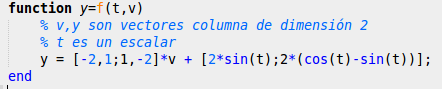
\includegraphics[width=\textwidth]{img/f.png}
    \end{minipage}
    \begin{minipage}{.4\textwidth}
        \centering
        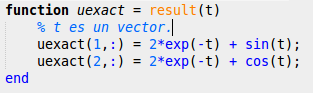
\includegraphics[width=\textwidth]{img/result.png}
    \end{minipage}
\end{center}

Una vez tenemos estas funciones definidas, procedemos a implementar el propio método de Euler, que podemos ver en la siguiente imagen.

\begin{center}
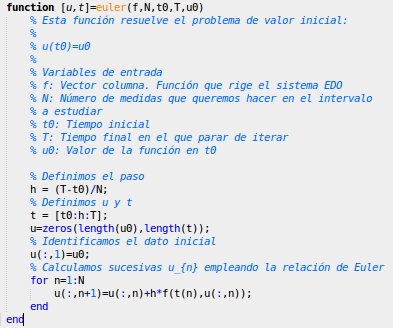
\includegraphics[width=0.6\textwidth]{img/euler.png}
\end{center}

Por último sólo tenemos que crear un programa principal que, llamando a las funciones ya definidas, resuelva el PVI planteado al inicio de esta sección.

\begin{center}
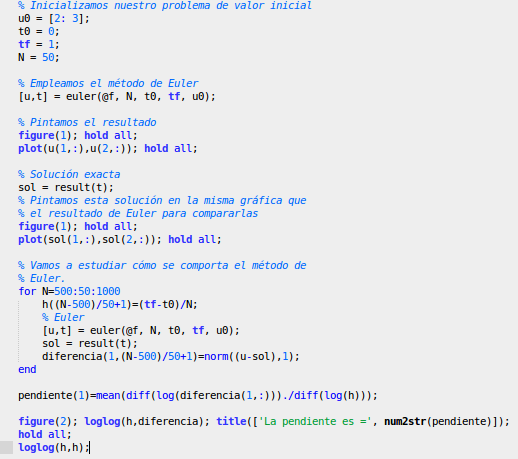
\includegraphics[width=0.8\textwidth]{img/aplicacion_euler.png}
\end{center}

Vamos a explicar detenidamente qué se está haciendo en este código. Para empezar estamos simplemente resolviendo el problema aplicando el método de Euler y pintando, en una misma gráfica, la solución dada por el método y la solución real, con lo que podemos observar la gran precisión de la solución obtenida por este método.
\begin{center}
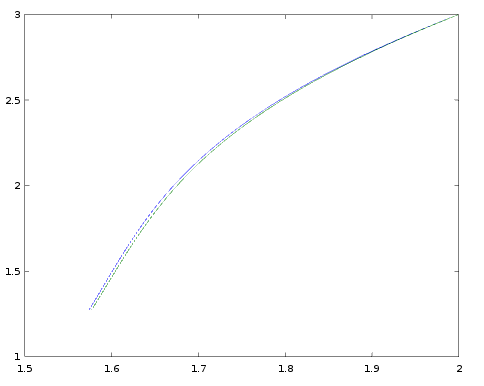
\includegraphics[width=0.8\textwidth]{img/figure1.png}
\end{center}

La última parte del código es la más compleja. Lo se está haciendo ahí es llamar numerosas veces al método de Euler y guardar, en cada llamada, la diferencia entre la función obtenida y la solución así como el $h$ empleado en esa ocasión.

Posteriormente calculamos la pendiente de la función que representan los pares de valores que hemos guardado. Para ello tomamos escala logarítmica y estudiamos la pendiente de la función en cada punto para, finalmente, tomar la media de esos valores.

Por último, pintamos estos valores junto con una función claramente lineal, que es $h$ con respecto a $h$ y obtenemos la siguiente gráfica.

\begin{center}
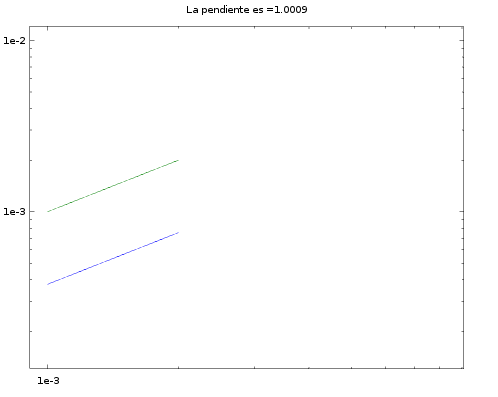
\includegraphics[width=0.8\textwidth]{img/figure2.png}
\end{center}

Ahora la pregunta que nos surge es clara, \textbf{¿por qué es interesante esta pendiente?}.

La idea se basa en el hecho de haber trabajado con logaritmos de los valores y no con los valores directamente. En general sabemos que el error se comporta como $e \leq c h^p$ para una cierta constante $c$, donde $p$ es el orden del método. Evidentemente podemos aplicar logaritmos a ambos lados sin que nada se estropee, obteniendo:
\[\log(e) \leq p \log(ch)\]

Si ahora dibujásemos la gráfica que relaciona el logaritmo del error con el logaritmo de $h$ obtendremos una recta con pendiente $p$ que es justo el \textbf{orden del método}.

Por tanto, esa pendiente que hemos calculado en el código, nos permite conocer el orden del método de Euler.
\end{document}



